
\documentclass[a4paper,11pt]{article}
\usepackage[left=2cm, right=2cm, top=2cm]{geometry}
\usepackage{amsmath}
\usepackage{amsthm}
\usepackage{amssymb}
\usepackage{amsfonts}
\usepackage[colorlinks = true]{hyperref}
\usepackage{graphicx}
\usepackage{float}
\usepackage{needspace}
\usepackage{fancyhdr}
\usepackage{color,xcolor}
\usepackage{enumitem}
\usepackage{longtable,array,booktabs}
\usepackage{setspace}
\usepackage{xcolor}
\usepackage{xepersian}
\usepackage{mathtools}
\usepackage{flexisym}
\usepackage{fontspec}


\IfFontExistsTF{XB Niloofar}{
  \settextfont{XB Niloofar}
  \setdigitfont{XB Niloofar}
  \setlatintextfont{XB Niloofar}
}{
  \settextfont{Amiri}
  \setdigitfont{Amiri}
  \setlatintextfont{Amiri}
}
\setmonofont{DejaVu Sans Mono}

\newcommand{\Code}[1]{\lr{\texttt{\detokenize{#1}}}}
\newcommand{\En}[1]{\lr{#1}}
\newcommand{\Num}[1]{\ifmmode\text{\lr{#1}}\else\lr{#1}\fi}
\graphicspath{{reports/}{figures/}{../figures/}}
\setstretch{1.19}
\setlength{\parindent}{0pt}\setlength{\emergencystretch}{2em}
\setlength{\parskip}{0.35em}
\renewcommand{\arraystretch}{1.23}
\hypersetup{hidelinks,pdfauthor={NACC Dataset C -- Statistics Course},pdftitle={Phase 2 NACC UDS and MRI}}
\begin{document}

\thispagestyle{fancy}
\fancyhf{}
\lhead{

 
\includegraphics[width=3cm]{reports/logo.png}
 \vspace{-2pt}
}
\chead{\leavevmode{\Huge به نام خدا}\vspace{15pt}\\  {\Large علیرضا جنتی}\vspace{10pt}\\{\small 403101672}\vspace{5pt}}
\rhead{

  {\large   پروژه درس آمار}

\vspace{10pt}   

{\large  فاز دوم}

\vspace{10pt}

ترم 14051
\vspace{-7pt}

}
\cfoot{\thepage}

\leavevmode
\vspace{20pt}


\vspace{1cm}

\begingroup
\hypersetup{linkcolor=blue}
\tableofcontents
\pagenumbering{gobble}
\endgroup
\clearpage
\pagenumbering{arabic} 
\pagebreak

\section{داده، متغیرها و تعریف رویدادها}
\subsection*{واحد مشاهده و کنترل مراجعات}

در فایل‌های تحویلی UDS و MRI هر فایل شامل ۱۲۳۷ ردیف
و ۱۲۳۷ شناسه یکتای \Code{NACCID} است. شناسه‌های دو فایل
کاملا با یکدیگر تطابق دارند و اتصال آن‌ها با رابطه یک‌به‌یک
انجام شده است. بنابراین هر شرکت‌کننده در محاسبات این فاز
دقیقا یک بار وارد شده است.

این قاعده صرفا ساختار زیرمجموعه آماده‌شده درسی را توصیف
می‌کند و به معنی وجود تنها یک مراجعه برای هر فرد در پایگاه
اصلی NACC نیست. از آنجا که شماره و تاریخ مراجعات UDS و
تاریخ اسکن MRI در فایل‌های تحویلی موجود نیستند، تعیین اینکه
رکورد انتخاب‌شده مربوط به مراجعه اولیه، آخرین مراجعه یا
نزدیک‌ترین مراجعه به زمان MRI است، امکان‌پذیر نیست.
در نتیجه، در این فاز انتخاب مجدد مراجعه انجام نشده و
از همان یک رکورد موجود برای هر \Code{NACCID} استفاده شده است.
\small
\begin{longtable}{p{5.0cm} p{5.0cm} p{4.0cm}}
\toprule
متغیر & تعریف و منبع & نوع و نقش \\
\midrule
\endfirsthead
\toprule
متغیر & تعریف و منبع & نوع و نقش \\
\midrule
\endhead
\Code{CDRSUM} & نمره مجموع جعبه‌های CDR از UDS & کمی گسسته؛ متغیر شناختی X \\
\Code{ENTORHINAL_MEAN_AVGTH} & میانگین ضخامت چپ و راست از MRI & کمی پیوسته؛ متغیر MRI به‌نام Y \\
\Code{NACCUDSD} & وضعیت شناختی UDS کد ۴ برابر دمانس & طبقه‌ای؛ تعریف رویداد A \\
\Code{NACCID} & شناسه شرکت‌کننده & کلید اتصال؛ نه متغیر تحلیلی \\
\bottomrule
\end{longtable}
\normalsize

رویداد :A فرد در طبقه دمانس وضعیت شناختی UDS قرار داشته باشد؛ یعنی
\Code{NACCUDSD = 4}.

رویداد :B میانگین ضخامت انتورینال دوطرفه کمتر از میانه فاز اول، یعنی
\Num{3.0575} باشد. مقدار مساوی آستانه در گروه \En{NOT B} قرار گرفته است.
در این داده \Num{2} نفر دقیقا برابر آستانه هستند. 

\textbf{تعداد افراد معتبر:} \Num{1,237} نفر؛ برای هر نفر مقدار معتبر \Code{CDRSUM} و هر دو ضخامت
انتورینال موجود است. هیچ فردی برای تحلیل‌های این فاز حذف نشده است.


\section{احتمال‌های حاشیه‌ای، مشترک و شرطی}
احتمال تجربی هر رویداد از نسبت فراوانی آن به تعداد افراد معتبر محاسبه شده است:
\[
P_{emp}(E)=\frac{n(E)}{N},\qquad N=\Num{1,237}.
\]
بنابراین درصدهای این بخش فقط فراوانی نسبی در زیرمجموعه درسی هستند و برآورد شیوع در جمعیت
عمومی محسوب نمی‌شوند.

\subsection*{احتمال‌های حاشیه‌ای}
\small
\begin{longtable}{ p{6cm} p{3cm} r }
\toprule
رویداد & فراوانی / کل & احتمال تجربی \\
\midrule
\endfirsthead
\toprule
رویداد & فراوانی / کل & احتمال تجربی \\
\midrule
\endhead
\(A\) & \En{131/1237} & \Num{10.5901\%} \\
\(\mathrm{NOT}\ A\) & \En{1106/1237} & \Num{89.4099\%} \\
\(B\) & \En{618/1237} & \Num{49.9596\%} \\
\(\mathrm{NOT}\ B\) & \En{619/1237} & \Num{50.0404\%} \\
\bottomrule
\end{longtable}
\normalsize
\subsection*{جدول توافق دو رویداد}
\small
\begin{longtable}{ p{4.2cm} r r r r }
\toprule
رویداد & \(B\) & \(\mathrm{NOT}\ B\) & مجموع & احتمال حاشیه‌ای \\
\midrule
\endfirsthead
\toprule
رویداد & \(B\) & \(\mathrm{NOT}\ B\) & مجموع & احتمال حاشیه‌ای \\
\midrule
\endhead
\En{A} & \Num{109} & \Num{22} & \Num{131} & \Num{10.59\%} \\
\En{NOT A} & \Num{509} & \Num{597} & \Num{1106} & \Num{89.41\%} \\
\En{Total} & \Num{618} & \Num{619} & \Num{1237} & \Num{100.00\%} \\
\bottomrule
\end{longtable}
\normalsize
 چهار خانه جدول مشترک به‌صورت زیر هستند:
\small
\begin{longtable}{ p{6cm} r r }
\toprule
رویداد مشترک & فراوانی & احتمال تجربی \\
\midrule
\endfirsthead
\toprule
رویداد مشترک & فراوانی & احتمال تجربی \\
\midrule
\endhead
\(A\cap B\) & \Num{109} & \Num{8.8116\%} \\
\(A\cap \mathrm{NOT}\ B\) & \Num{22} & \Num{1.7785\%} \\
\(\mathrm{NOT}\ A\cap B\) & \Num{509} & \Num{41.1479\%} \\
\(\mathrm{NOT}\ A\cap \mathrm{NOT}\ B\) & \Num{597} & \Num{48.2619\%} \\
\bottomrule
\end{longtable}
\normalsize
\enlargethispage{5pt}
\subsection*{احتمال‌های شرطی}
\small
\begin{longtable}{ p{5cm} p{4cm} r }
\toprule
احتمال شرطی & صورت / مخرج & درصد \\
\midrule
\endfirsthead
\toprule
احتمال شرطی & صورت / مخرج & درصد \\
\midrule
\endhead
\(P(A\mid B)\) & \En{109/618} & \Num{17.6375\%} \\
\(P(A\mid \mathrm{NOT}\ B)\) & \En{22/619} & \Num{3.5541\%} \\
\bottomrule
\end{longtable}
\normalsize

\textbf{تفسیر:} در گروه دارای ضخامت کمتر از میانه، احتمال تجربی وضعیت دمانس UDS برابر
\Num{17.64\%} است؛ در گروه دارای ضخامت مساوی یا بیشتر از میانه این مقدار
\Num{3.55\%} است. این دو احتمال شرطی نشان می‌دهند که محدودکردن محاسبه
به گروه MRI، فراوانی نسبی رویداد A را تغییر می‌دهد. این مقایسه توصیفی است و به‌تنهایی آزمون
معناداری یا رابطه علّی محسوب نمی‌شود.

\begin{figure}[H]
\centering
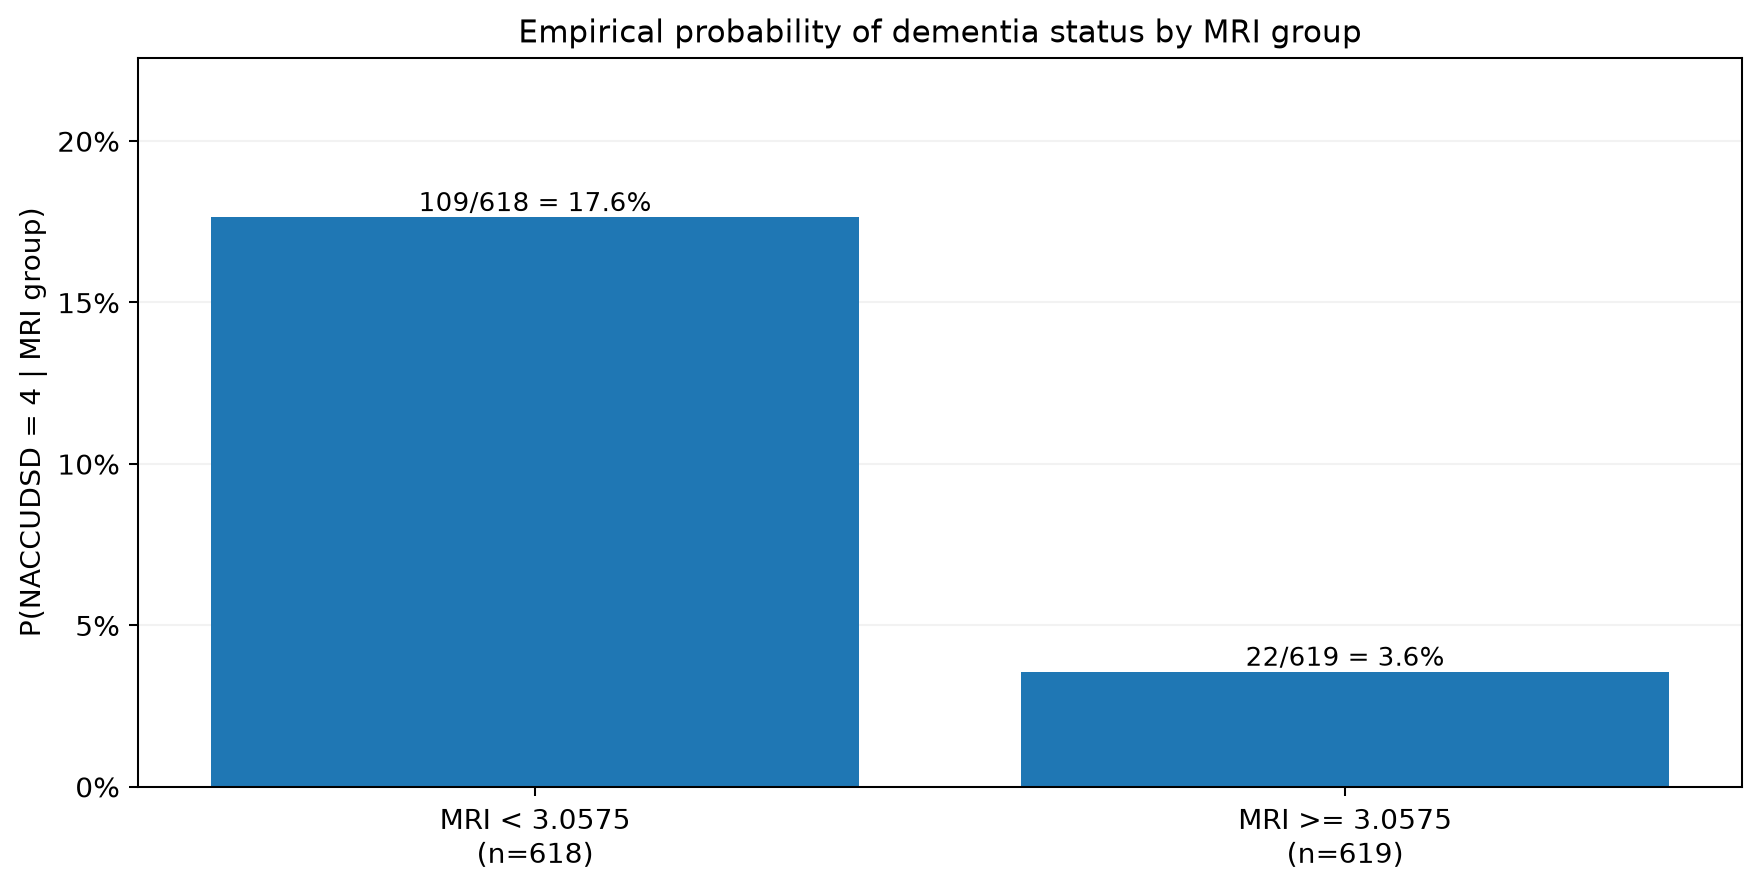
\includegraphics[width=.72\linewidth]{phase2_01_conditional_cognitive_status.png}
\caption{احتمال تجربی وضعیت دمانس UDS در دو گروه تعریف‌شده با میانه MRI.}
\end{figure}

\section{استقلال رویدادها}
برای استقلال A و B باید رابطه زیر برقرار باشد:
\[
P(A\cap B)=P(A)P(B).
\]
در داده حاضر، احتمال مشترک مشاهده‌شده برابر \Num{8.8116\%} و حاصل‌ضرب
احتمال‌های حاشیه‌ای برابر \Num{5.2908\%} است. اختلاف این دو مقدار
\Num{3.5209} واحد درصد است.

\textbf{نتیجه:} فراوانی‌های تجربی این زیرمجموعه با استقلال A و B سازگار به نظر نمی‌رسند.

\section{متغیر برنولی، مدل دوجمله‌ای و قضیه بیز}
\subsection*{متغیر برنولی و توزیع دوجمله‌ای}
متغیر دودویی زیر برای رویداد A تعریف شد:
\[
Z=\begin{cases}1 & A\\0 & \mathrm{NOT}\ A.\end{cases}
\]
پارامتر تجربی آن برابر \(p=131/1237=\Num{0.105901}\) است. برای توضیح رفتار یک شمارش
دودویی، تعداد رخداد A در ۱۰ انتخاب فرضی و مستقل با K نشان داده شد:
\[
K\sim Binomial(n=10,p),\qquad P(K=k)=\binom{10}{k}p^k(1-p)^{10-k}.
\]
\small
\begin{longtable}{ r r }
\toprule
تعداد رخداد A (k) & \(P(K=k)\) \\
\midrule
\endfirsthead
\toprule
تعداد رخداد A (k) & \(P(K=k)\) \\
\midrule
\endhead
\Num{0} & \Num{0.326478} \\
\Num{1} & \Num{0.386697} \\
\Num{2} & \Num{0.206110} \\
\Num{3} & \Num{0.065100} \\
\Num{4} & \Num{0.013494} \\
\Num{5} & \Num{0.001918} \\
\Num{6} & \Num{0.000189} \\
\Num{7} & \Num{1.281e-05} \\
\Num{8} & \Num{5.691e-07} \\
\Num{9} & \Num{1.498e-08} \\
\Num{10} & \Num{1.770e-10} \\
\bottomrule
\end{longtable}
\normalsize

جدول بالا تابع جرم احتمال شمار رخداد A را برای تمام مقادیر ممکن K در ده انتخاب فرضی نشان می‌دهد.

\textbf{محدودیت مدل:} ده انتخاب در اینجا یک مثال نظری است و به معنی نمونه‌گیری واقعی ده نفر
از NACC نیست. برای نمونه‌گیری بدون جایگذاری از یک مجموعه محدود، مدل دقیق فوق‌هندسی است؛
مدل دوجمله‌ای فقط در صورت ثابت‌بودن احتمال و استقلال انتخاب‌ها مناسب است. نسبت ۱۰ به ۱۲۳۷
حدود \Num{0.81\%} است، اما در فایل‌های تحویلی طرح نمونه‌گیری تصادفی برای این ده انتخاب ثبت نشده؛
پس مدل صرفا برای نمایش توزیع دوجمله‌ای به‌کار رفته است.

\begin{figure}[H]
\centering
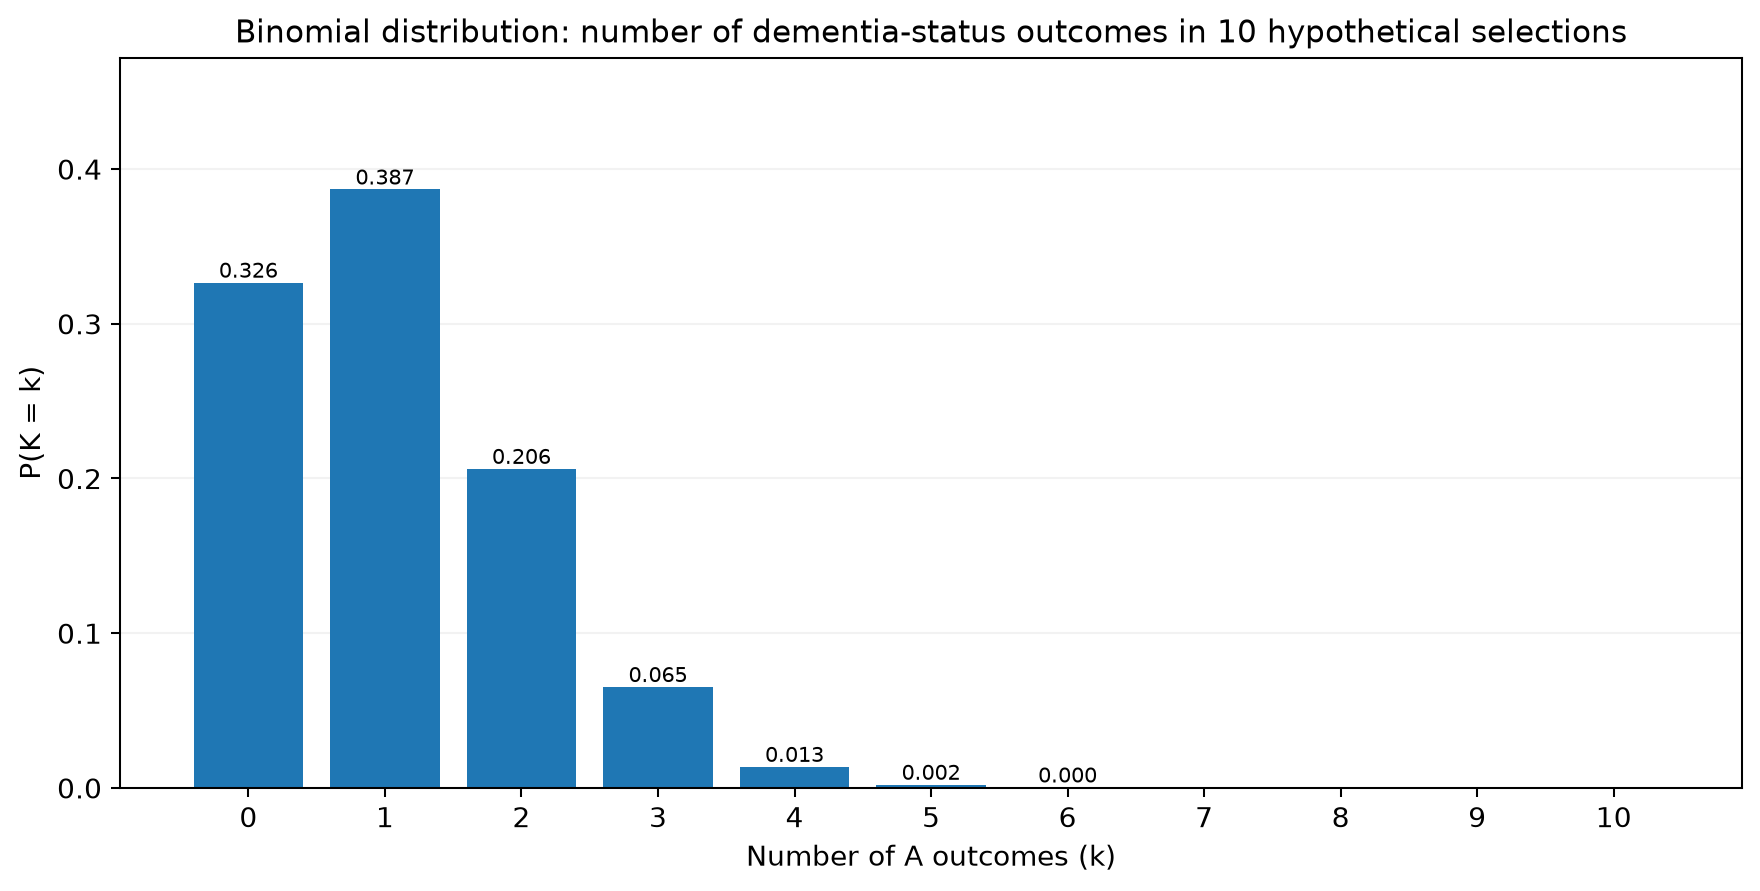
\includegraphics[width=.82\linewidth]{phase2_02_binomial_pmf.png}
\caption{تابع جرم احتمال شمار رخداد A در ده انتخاب فرضی مستقل.}
\end{figure}

\subsection*{قضیه بیز}
برای دو رویداد تعریف‌شده، به‌روزرسانی احتمال با قضیه بیز به شکل زیر است:
\[
P(A|B)=\frac{P(B|A)P(A)}{P(B)}.
\]
با جایگذاری فراوانی‌های تجربی، مقدار بیزی برابر \Num{17.6375\%} به دست آمد؛
احتمال شرطی مستقیم مرحله اول نیز \Num{17.6375\%} است.

\section{توزیع، امید ریاضی، واریانس و نقاط دورافتاده}
برای هر دو متغیر، توزیع تجربی، میانگین و واریانس محاسبه شد. چارک‌ها با درون‌یابی خطی محاسبه شده‌اند.

\small
\begin{longtable}{ p{7.2cm} r r }
\toprule
شاخص توصیفی & \Code{CDRSUM} & میانگین ضخامت MRI \\
\midrule
\endfirsthead
\toprule
شاخص توصیفی & \Code{CDRSUM} & میانگین ضخامت MRI \\
\midrule
\endhead
تعداد معتبر & \Num{1237} & \Num{1237} \\
میانگین & \Num{0.8222} & \Num{3.0138} \\
واریانس تجربی با مخرج N & \Num{2.9663} & \Num{0.1267} \\
انحراف معیار نمونه‌ای با مخرج N-1 & \Num{1.7230} & \Num{0.3561} \\
میانه & \Num{0.0000} & \Num{3.0575} \\
چارک اول Q1 & \Num{0.0000} & \Num{2.8025} \\
چارک سوم Q3 & \Num{1.0000} & \Num{3.2515} \\
دامنه & \Num{0.000} تا \Num{15.000} & \Num{1.214} تا \Num{3.925} \\
تعداد نقاط خارج از حصار IQR & \Num{115} & \Num{22} \\
\bottomrule
\end{longtable}
\normalsize

میانگین \Code{CDRSUM}، متوسط نمره در همین زیرمجموعه را نشان می‌دهد؛ واریانس \Num{2.9663}
با واحد امتیاز به توان دو، پراکندگی نمره‌ها را حول این میانگین خلاصه می‌کند. برای متغیر MRI،
میانگین ضخامت \Num{3.0138} میلی‌متر فرض‌شده و واریانس \Num{0.1267}
میلی‌متر به توان دو است؛ انحراف معیار نمونه‌ای \Num{0.3561} میلی‌متر، مقیاس پراکندگی را
در واحد اصلی متغیر نشان می‌دهد.

نمره CDRSUM: مقدار صفر برای \Num{757} نفر، یعنی \Num{61.20\%} از زیرمجموعه، ثبت شده است.
توزیع به‌شدت راست‌چوله است. با توجه به \(Q_1=0\)، \(Q_3=1\) و \(IQR=1\)،
حصارهای IQR از \Num-1.5 تا \Num2.5 هستند؛ \Num{115} مقدار بالاتر از حصار بالا قرار می‌گیرند.
برای این متغیر گسسته، تقریب نرمال توصیف مناسبی از توزیع کامل نیست.

متغیر MRI: میانگین ضخامت دوطرفه \Num{3.0138} و میانه آن \Num{3.0575} است.
میانگین کمتر از میانه است و چولگی تجربی برابر \Num{-0.817} است. این شاخص
توصیفی با عدم تقارن به سمت مقادیر پایین سازگار است؛ نمودار Q-Q نیز انحراف دنباله پایین را نشان می‌دهد.

قاعده نقاط دورافتاده: نقاط خارج از حصارهای \(Q_1-1.5IQR\) و \(Q_3+1.5IQR\)
پرچم‌گذاری شده‌اند. برای \Code{CDRSUM} حصارها از \Num{-1.500} تا
\Num{2.500} هستند؛ برای MRI از \Num{2.129} تا
\Num{3.925}. تعداد نقاط پرچم‌خورده به‌ترتیب \Num{115} و
\Num{22} است. این پرچم‌ها به‌معنی خطای قطعی داده نیستند؛ هیچ فرد یا
مقداری به دلیل دورافتاده‌بودن حذف نشده است.

\subsection*{توزیع تجربی کامل CDRSUM}
\small
\begin{longtable}{ r r r }
\toprule
نمره CDRSUM & تعداد & درصد \\
\midrule
\endfirsthead
\toprule
نمره CDRSUM & تعداد & درصد \\
\midrule
\endhead
\Num{0.0} & \Num{757} & \Num{61.20\%} \\
\Num{0.5} & \Num{144} & \Num{11.64\%} \\
\Num{1.0} & \Num{97} & \Num{7.84\%} \\
\Num{1.5} & \Num{50} & \Num{4.04\%} \\
\Num{2.0} & \Num{39} & \Num{3.15\%} \\
\Num{2.5} & \Num{35} & \Num{2.83\%} \\
\Num{3.0} & \Num{20} & \Num{1.62\%} \\
\Num{3.5} & \Num{12} & \Num{0.97\%} \\
\Num{4.0} & \Num{14} & \Num{1.13\%} \\
\Num{4.5} & \Num{21} & \Num{1.70\%} \\
\Num{5.0} & \Num{10} & \Num{0.81\%} \\
\Num{5.5} & \Num{3} & \Num{0.24\%} \\
\Num{6.0} & \Num{9} & \Num{0.73\%} \\
\Num{6.5} & \Num{1} & \Num{0.08\%} \\
\Num{7.0} & \Num{5} & \Num{0.40\%} \\
\Num{8.0} & \Num{9} & \Num{0.73\%} \\
\Num{9.0} & \Num{5} & \Num{0.40\%} \\
\Num{11.0} & \Num{2} & \Num{0.16\%} \\
\Num{12.0} & \Num{1} & \Num{0.08\%} \\
\Num{13.0} & \Num{1} & \Num{0.08\%} \\
\Num{14.0} & \Num{1} & \Num{0.08\%} \\
\Num{15.0} & \Num{1} & \Num{0.08\%} \\
\bottomrule
\end{longtable}
\normalsize

\begin{figure}[H]
\centering
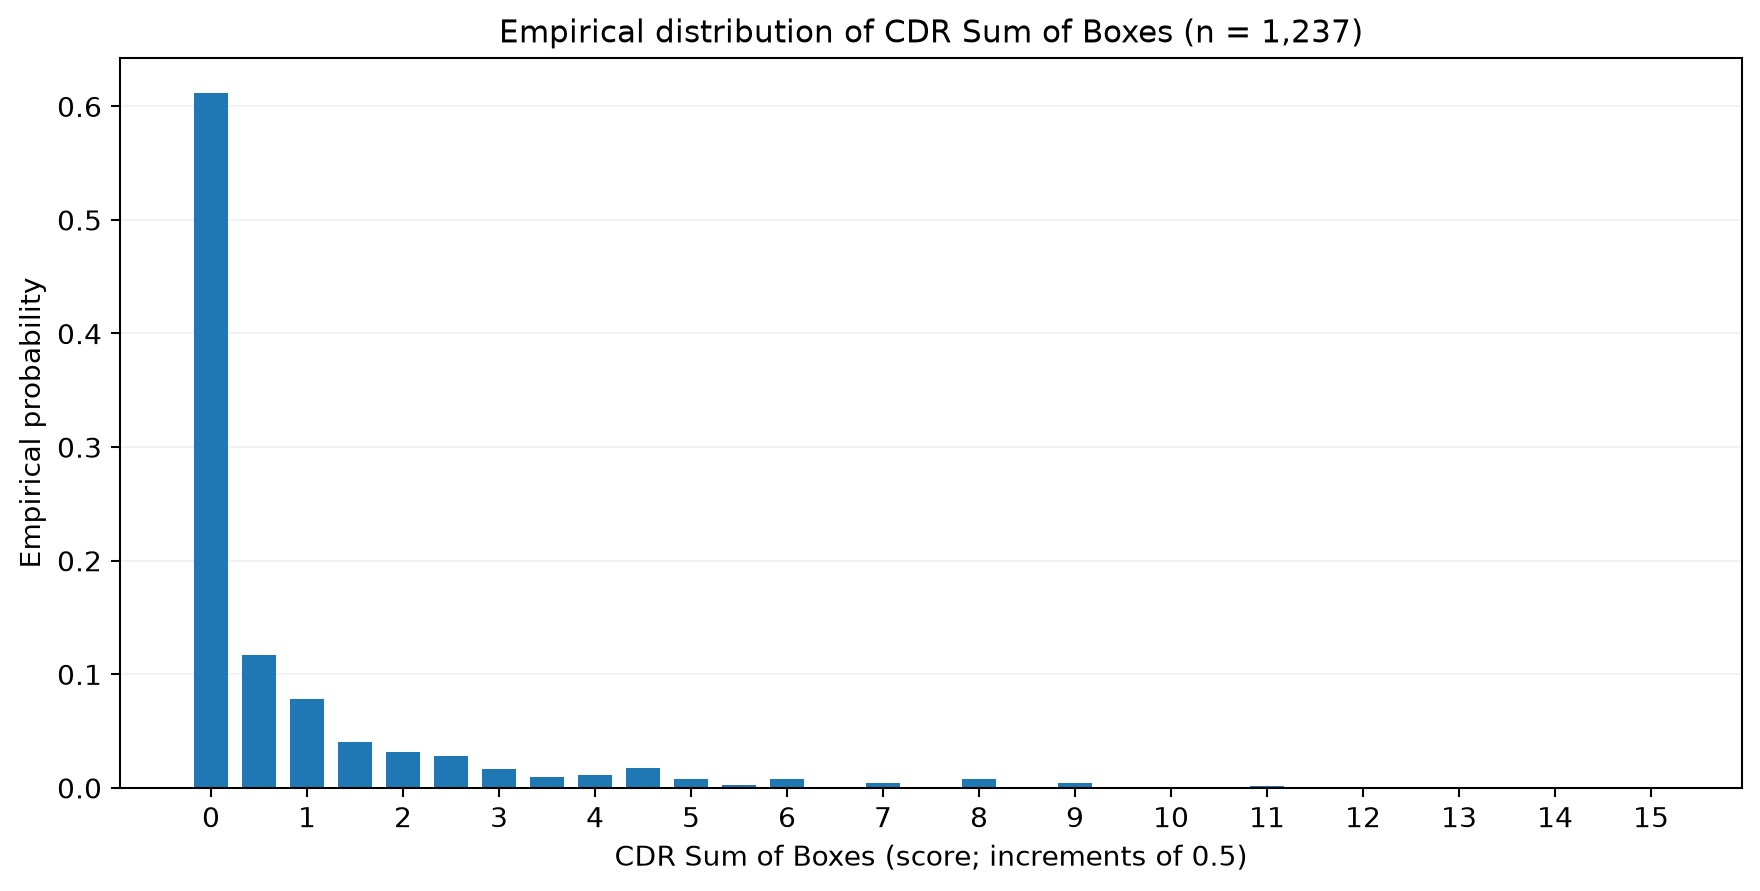
\includegraphics[width=.82\linewidth]{phase2_03_cdrsum_distribution.png}
\caption{توزیع تجربی گسسته نمره CDRSUM.}
\end{figure}

\subsection*{بررسی تقریب نرمال برای متغیر پیوسته MRI}
برای متغیر پیوسته ضخامت انتورینال، هیستوگرام همراه منحنی نرمال مرجع و نمودار کوانتایل--کوانتایل
بررسی شد. این دو نمودار برای ارزیابی بصری شکل توزیع استفاده شده‌اند؛ آزمون رسمی نرمال‌بودن
اجرا نشده است.

\begin{figure}[H]
\centering
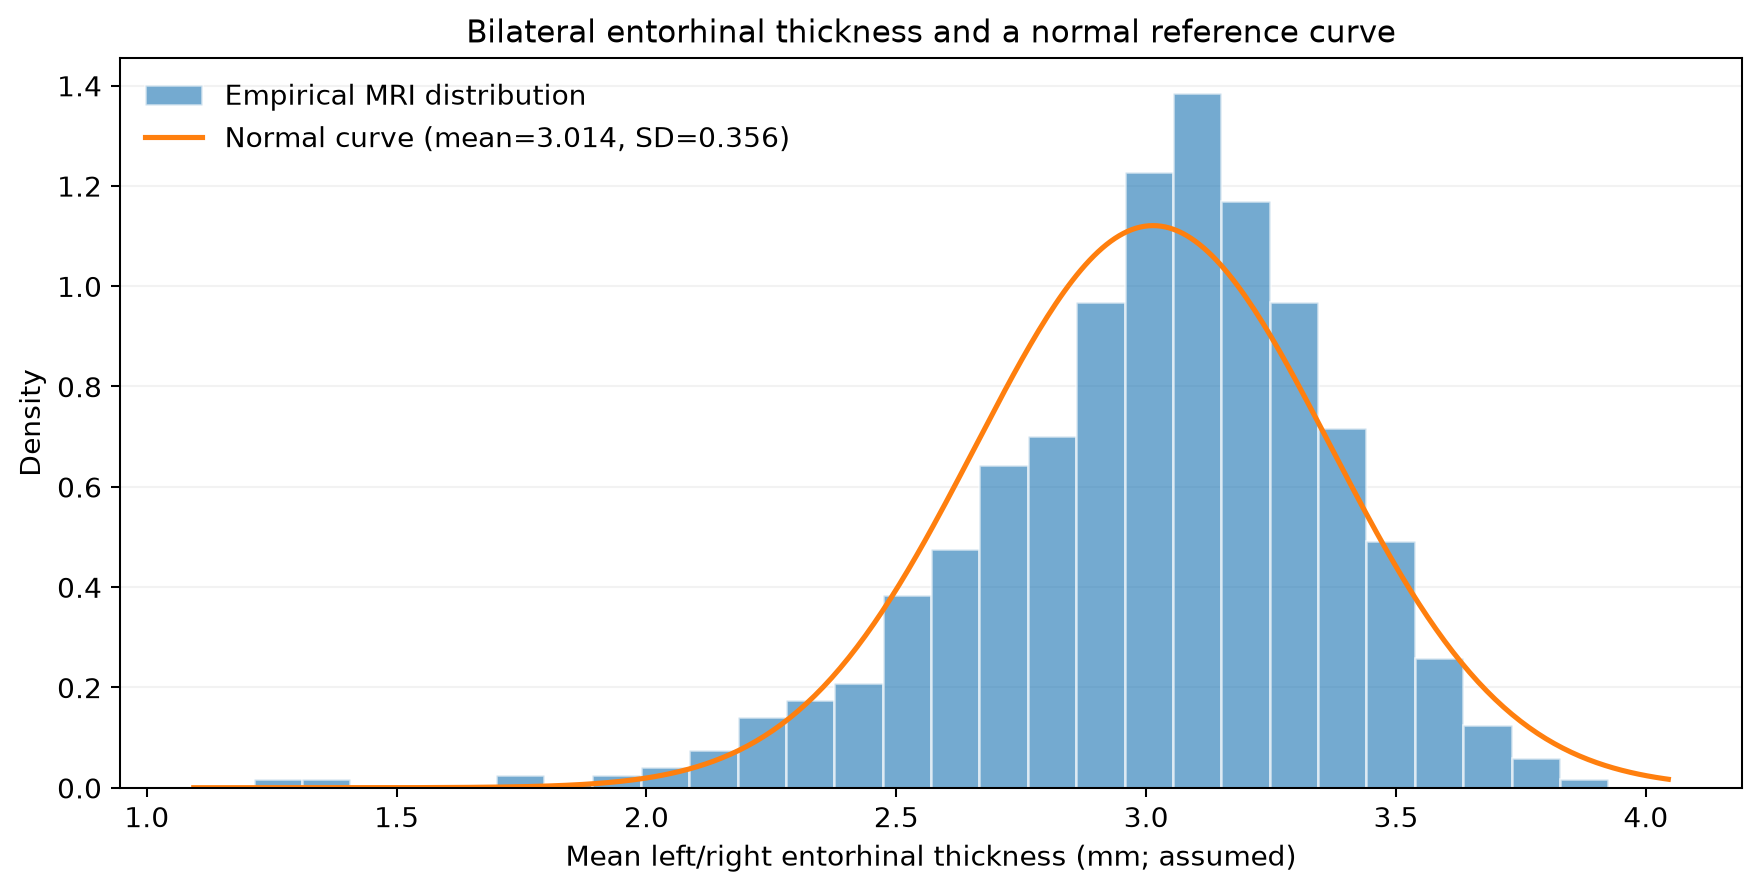
\includegraphics[width=.82\linewidth]{phase2_04_mri_thickness_distribution.png}
\caption{هیستوگرام ضخامت انتورینال دوطرفه و منحنی نرمال مرجع با میانگین و انحراف معیار تجربی.}
\end{figure}

\begin{figure}[H]
\centering
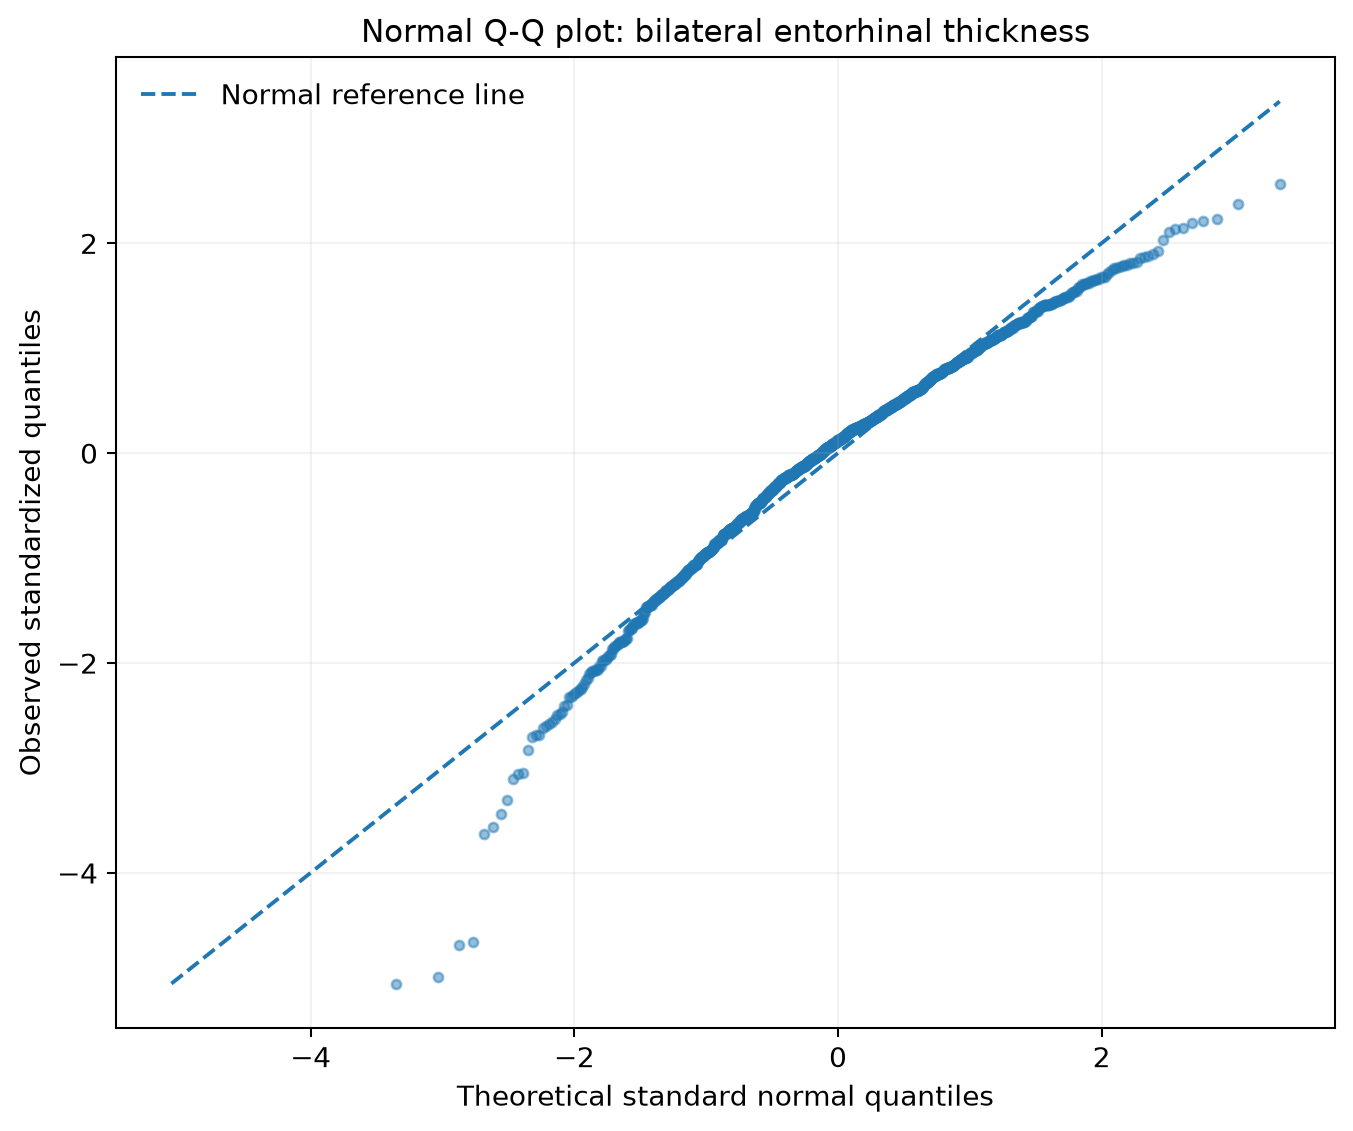
\includegraphics[width=.75\linewidth]{phase2_05_mri_normal_qq.png}
\caption{نمودار Q-Q برای بررسی انحراف توزیع ضخامت MRI از توزیع نرمال.}
\end{figure}

بر اساس نمودارها، بخش مرکزی توزیع تا حدی به خط مرجع نزدیک است، اما دنباله پایین انحراف
مشخصی دارد و \Num{22} مقدار پایین‌تر از حصار IQR قرار گرفته‌اند. بنابراین منحنی نرمال، توصیف کاملی
از کل توزیع نیست و باید با احتیاط به‌عنوان تقریب استفاده شود.

\section{کوواریانس شناخت و تصویربرداری}
برای دو متغیر کمی اصلی، \(X=CDRSUM\) و \(Y=ENTORHINAL\_MEAN\_AVGTH\)، کوواریانس تجربی
با مخرج \(N\) محاسبه شد:
\[
Cov_{emp}(X,Y)=\frac{1}{N}\sum_{i=1}^{N}(X_i-\bar X)(Y_i-\bar Y).
\]

مقدار به‌دست‌آمده برابر است با:
\[
Cov_{emp}(X,Y)=\Num{-0.178813}.
\]
علامت منفی نشان می‌دهد در این زیرمجموعه، مقادیر بالاتر از میانگین \Code{CDRSUM} تمایل دارند
همراه با مقادیر پایین‌تر از میانگین ضخامت انتورینال دیده شوند. واحد کوواریانس «امتیاز CDR
ضرب‌در میلی‌متر فرضی» است و مقدار آن به مقیاس دو متغیر وابسته است. در این فاز ضریب همبستگی
یا رگرسیون محاسبه نشده و از کوواریانس نتیجه علّی گرفته نمی‌شود.

\begin{figure}[H]
\centering
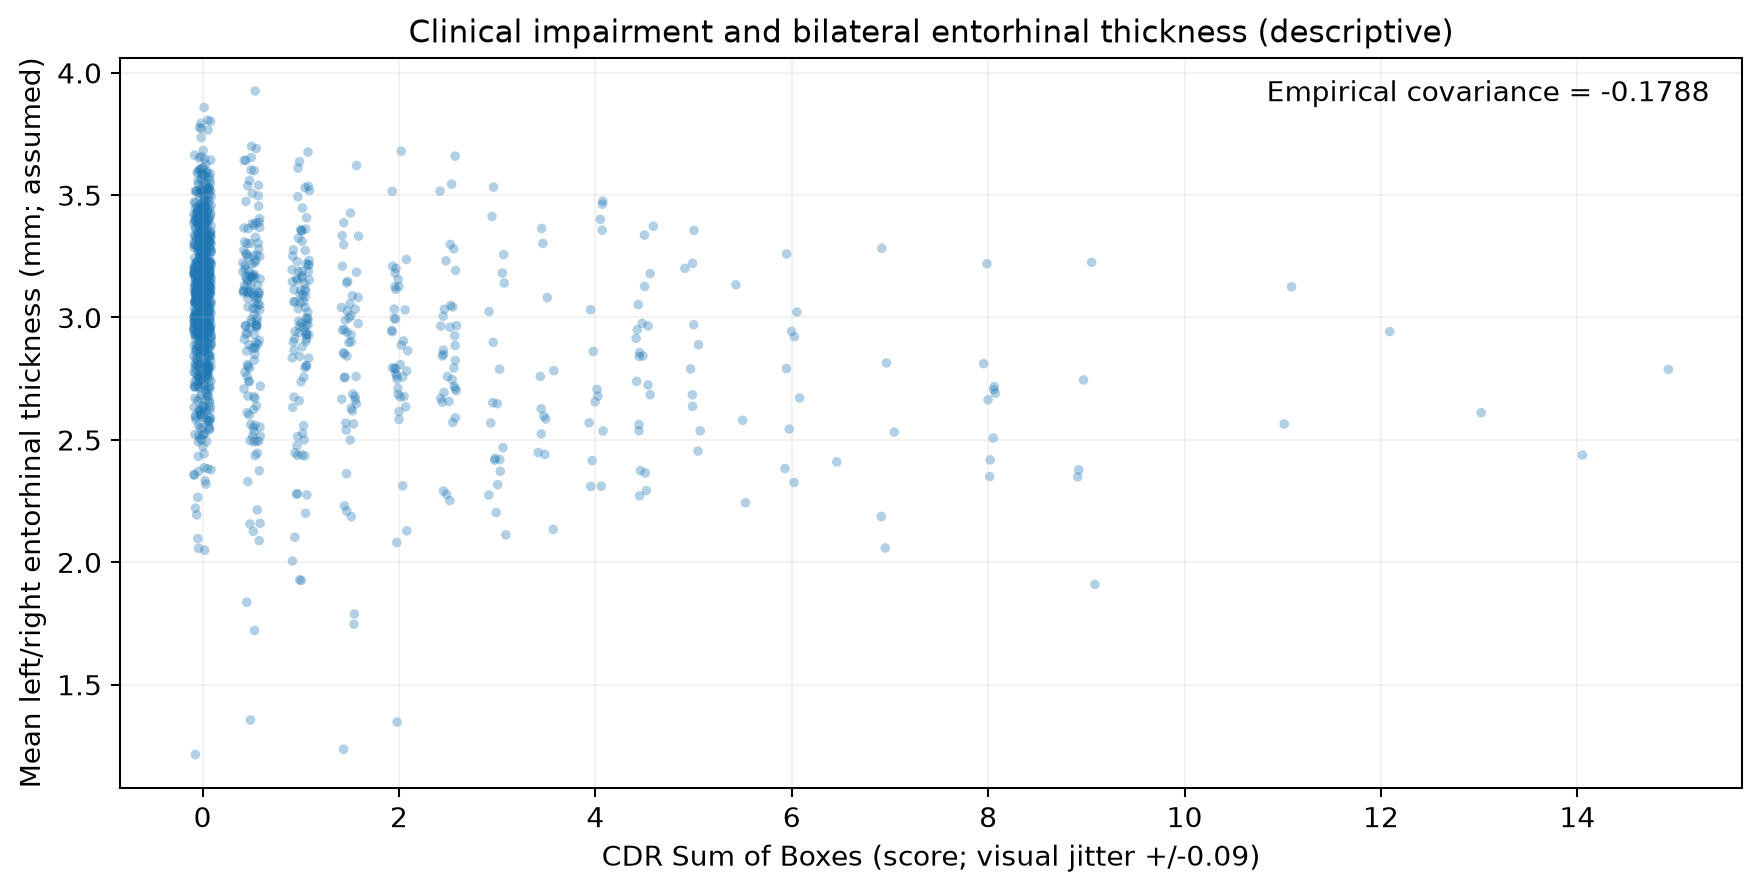
\includegraphics[width=.82\linewidth]{phase2_06_cdrsum_mri_covariance.png}
\caption{نمودار پراکنش جفت‌های واقعی CDRSUM و ضخامت دوطرفه؛ جابه‌جایی افقی صرفا برای نمایش نقاط هم‌پوشان است.}
\end{figure}


\section{بحث، محدودیت‌ها و جمع‌بندی}
در زیرمجموعه ۱۲۳۷ نفری، احتمال تجربی وضعیت دمانس UDS در گروه MRI زیر میانه بیشتر از گروه
مساوی یا بالاتر از میانه است. مقایسه احتمال‌های مشترک و حاصل‌ضرب احتمال‌های حاشیه‌ای نیز
با استقلال رویدادهای تعریف‌شده سازگار نیست. مدل دوجمله‌ای و قضیه بیز، روابط احتمالی را با
همان فراوانی‌های تجربی روشن می‌کنند.

توزیع \Code{CDRSUM} دارای تراکم زیاد در صفر و چولگی راست است. توزیع ضخامت انتورینال دوطرفه
در بخش مرکزی تا حدی به منحنی نرمال نزدیک است، اما دنباله پایین و نقاط دورافتاده نشان می‌دهند
تقریب نرمال برای کل توزیع کامل نیست. کوواریانس منفی نیز جهت رابطه توصیفی بین شدت بالینی و
ضخامت انتورینال را نشان می‌دهد؛ اما اندازه آن به مقیاس متغیرها وابسته است.

\textbf{محدودیت‌ها:} این زیرمجموعه نمونه احتمالی از جمعیت عمومی نیست؛ فایل UDS از پیش
\En{imputed} شده و روش جایگذاری معلوم نیست؛ تاریخ MRI و ارزیابی UDS در دسترس نیست؛ واحد
میلی‌متر برای ضخامت فرض شده؛ وضعیت دمانس UDS علت آلزایمری را مشخص نمی‌کند. نقاط دورافتاده
حذف نشده‌اند و هیچ آزمون استنباطی یا نتیجه علّی ارایه نشده است.

\textbf{جمع‌بندی:} فاز دوم با تعریف ثابت رویدادها، محاسبه احتمال‌های تجربی و شرطی، بررسی
توصیفی استقلال، مدل دوجمله‌ای و قضیه بیز، توصیف توزیع دو متغیر اصلی و محاسبه کوواریانس
به پایان رسیده است. تحلیل‌های استنباطی و مدل‌سازی به فازهای بعدی موکول می‌شوند.

\subsection*{ردیابی تسک‌های رسمی فاز دوم}
جدول زیر محل پوشش هر ۹ تسک مشترک و ۵ الزام اختصاصی مسیر ج را در گزارش مشخص می‌کند.
\small
\begin{longtable}{p{2.0cm} p{9.0cm} r}
\toprule
تسک & موضوع & بخش گزارش \\
\midrule
\endfirsthead
\toprule
تسک & موضوع & بخش گزارش \\
\midrule
\endhead

مشترک ۱ & تعریف رویدادها و متغیرهای تصادفی & ۱ و ۴ \\
مشترک ۲ & احتمال‌های حاشیه‌ای و مشترک & ۲ \\
مشترک ۳ & احتمال شرطی & ۲ \\
مشترک ۴ & بررسی استقلال & ۳ \\
مشترک ۵ & توزیع گسسته و مدل دوجمله‌ای & ۴ \\
مشترک ۶ & متغیر پیوسته و تقریب نرمال & ۵ \\
مشترک ۷ & امید ریاضی و واریانس & ۵ \\
مشترک ۸ & دو متغیر تصادفی و کوواریانس & ۶ \\
مشترک ۹ & قضیه بیز & ۴ \\
ج.۱ & احتمال شرطی وضعیت شناختی & ۲ \\
ج.۲ & توزیع نمره شناختی و متغیر MRI & ۵ \\
ج.۳ & احتمال مشترک دو وجه & ۲ \\
ج.۴ & کوواریانس شناخت و تصویربرداری & ۶ \\
ج.۵ & کنترل مراجعات و یک مشاهده برای هر فرد & ۱ \\

\bottomrule
\end{longtable}

\end{document}
